\documentclass[10pt,oneside,openright, a4paper]{memoir}
\bibliographystyle{apalike}
\usepackage[T1]{fontenc}
\usepackage{listings}
\lstset{numbers=none,boxpos=c}
\usepackage{enumitem}
\usepackage{graphicx}
\usepackage{dirtree}
\usepackage{url}
\linespread{1.2}

\usepackage{amsmath,amssymb,amsfonts}% Typical maths resource packages
\usepackage{graphics}                % Packages to allow inclusion of graphics
\usepackage{color}                   % For creating coloured text and background
\usepackage{hyperref}                % For creating hyperlinks in cross references
\usepackage{listings}
\usepackage{wrapfig}
\usepackage{subfig}
\usepackage{float}
\usepackage{titling}
\usepackage[absolute]{textpos}      % Use option showboxes to see bounding areas
\usepackage[document]{ragged2e}

\setlrmarginsandblock{2cm}{2.5cm}{*}
\setulmarginsandblock{2cm}{2cm}{*}
\checkandfixthelayout

\fontfamily{erewhon}
\textwidth 15.5cm
\topmargin -1.5cm
\parindent 0cm
\textheight 24cm
\parskip 1mm

\begin{document}
\title{Introduction to Threadneedle}
\author{Jacky Mallett}
%\lstset{language=C++, basicstyle=\ttfamily\footnotesize, stringstyle=\sffamily\scriptsize\bfseries, commentstyle=\sffamily\small\bfseries }

%\pagestyle{myheadings}         % Option to put page headers


%\pagenumbering{}


%\author{
%\sffamily\Large I. B. Author \& U. B. Author \\ 
%\sffamily\small i.b.author@iiim.is, u.b.author@iiim.is\\ \\ \\
%\sffamily\Large Icelandic Institute for Intelligent Machines \\
%\sffamily\Large Menntavegur 1, 2.h. Uranus \\
%\sffamily\Large 101 Reykjavik, Iceland\\ \\ \\ \\ \\ \\ \\
%\sffamily\Large IIIM TECH REPORT IIIMTR-YEAR-MM-cnt\\   % MM = two-digit month;
%                               % cnt = three digit counter, counting
%                               % the number of TRs to come out at
%                               % IIIM that month
%}


% TITLEPAGE
%
% textblock package used for absolute positioning 
% http://www.tex.ac.uk/tex-archive/macros/latex/contrib/textpos/textpos.pdf
%
\begin{titlingpage}
\begin{textblock}{2}(0,0)
  {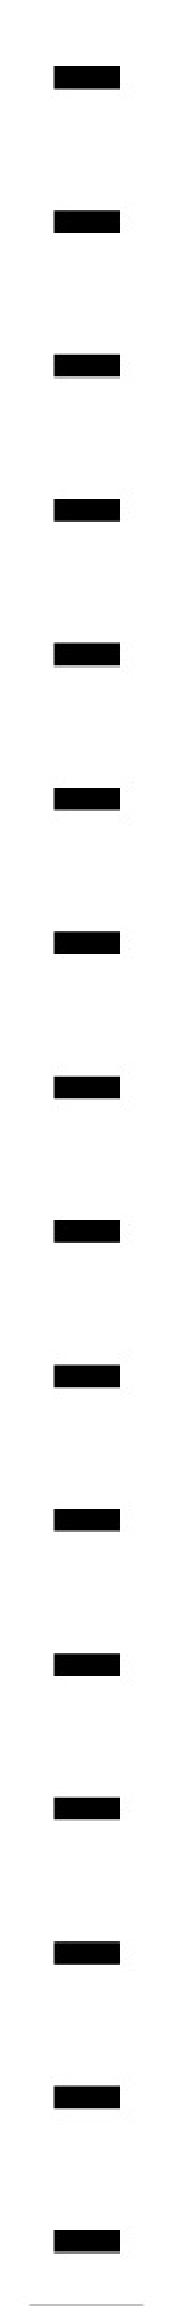
\includegraphics{iiim/IIIM-header-stripes-vertical.eps}}
\end{textblock}
\begin{textblock}{5}(11,1)
  {
\includegraphics[width=5cm]{iiim/IIIM-logo.eps}}
\end{textblock}
\begin{textblock}{8}(7,14.6) {IIIM TECH REPORT IIIMTR-2015-06-001}
\end{textblock}
\begin{textblock}{5}(12.4,14.5)
  {
\includegraphics[width=3cm]{iiim/wwwiiimis-black-box.eps}}
\end{textblock}
\begin{textblock}{5}(7,15.1)
   
\includegraphics[width=10.1cm]{iiim/IIIM-black-box.eps}
\end{textblock}

\begin{textblock}{10}(3,5)
{
\textbf{
\huge  
\thetitle \\ 
\vspace{2mm} 
\theauthor \\
\vspace{2mm} 
\small jacky@iiim.is \\
\vspace{5mm} 
\large Icelandic Institute for Intelligent Machines \\
\large Menntavegur 1, 2.h. Uranus \\
\large 101 Reykjavik, Iceland\\ 
\vspace{4mm} 
%IIIM
}}
\end{textblock}
\end{titlingpage}

 % INSERT PAPER CONTENT



\null\newpage
%%% BEGIN DOCUMENT

%\let\cleardoublepage\clearpage
%\maketitle
%\frontmatter
%\null\vfill
%\begin{flushleft}
%\textit{Introduction to Threadneedle}
%\copyright Jacky Mallett
%All rights reserved. 2015
%%ISBN--INFO
%%ISBN--13: 
%\bigskip
%\end{flushleft}
%\let\cleardoublepage\clearpage

\mainmatter
\sloppy
\chapter{Introduction}
Threadneedle is an economic simulation platform designed 
to support agent based research on modern financial systems 
using fractional reserve banking. At its core, Threadneedle
incorporates a full emulation of fractional reserve banking, 
implemented using double entry book keeping for all banking operations,
allowing financial systems to be constructed with a wide range of 
regulatory controls and financial instruments.
\par
The goal of Threadneedle is to provide a simulation environment in which 
individual economic agents can interact with each other using monetary 
transactions, identical to real world transactions, allowing
experiments to be performed on the impact of different combinations
of behaviours, regulatory controls, and financial constructs.
A base set of agents: individuals, companies, banks, markets and
Governments is supplied with the framework, and these are supported 
within an infrastructure which provides access to banking services for
all agents. These can be used both to build 
simple economies, and can also be extended to provide additional 
behaviours as researchers require.
\par
Agents in Threadneedle interact with each other solely through monetary 
signals provided by market pricing, taxation, lending and its associated 
interest rates, and the flow of money between individual agents as transactions
occur.  Within the constraints of fractional reserve banking, the regulatory 
structure surrounding the banking system can be configured to allow the 
exploration of different regulatory environments. Central bank reserve 
and Basel capital reserve regulatory frameworks are fully supported, but 
full reserve and free banking systems systems can 
also be created by imposing restrictions on the operations of the banks
within the simulation. 
\par
Threadneedle (version 1.0) is a research tool under active development, and 
is presented as such here. Some familiarity with Java and command line 
utilities is necessary in order  to install the package. Simple economic 
experiments can be performed with the set of base agents included, but most 
researchers will want
to enhance and extend these to provide richer simulations.
Those who wish to create new agents for the model or change behaviours will
need some programming experience with Java, and a programming guide is provided
to assist with this. (See the Programmer's Guide to Threadneedle for more information).
\par
Threadneedle is provided free for non-commercial research purposes under the creative commons Attribution-NonCommercial 4.0 License. Questions about licensing, 
comments, bug reports, suggestions, feature requests and/or code contributions,
should be sent to the author, Jacky Mallett(jacky@iiim.is). 
\chapter{Quick Start}
\section{Recommended Directory structure}
Install the Threadneedle class and java files in a top level
directory called Threadneedle.  The CLASSPATH environment variable 
for Java will need to be set to include this directory and the classes 
directory.
For example (linux, bash shell) if Threadneedle is in directory \textasciitilde/src/Threadneedle:
\begin{center}
\begin{tabular}{c}
\begin{lstlisting}
CLASSPATH=\$CLASSPATH:~/src/Threadneedle:~/src/Threadneedle/classes:
export CLASSPATH
\end{lstlisting}
\end{tabular}
\end{center}
In Windows, the CLASSPATH can be accessed as follows:
\begin{lstlisting}
Right Click Start
>  Click Control Panel  (Or you may have System in the list)
>  Click System
>  Click Advanced system settings
>  Go to the Advanced Tab
>  Click the "Environment Variables..." button at the bottom of that dialog page.
\end{lstlisting}
All the examples in this document are based on an installation using
the following file structure:
\par
\begin{figure}[ht]
\centering
\framebox[\textwidth]{%
\begin{minipage}{0.9\textwidth}
\dirtree{%
.1 src/.
.2 Threadneedle/.
.3 classes/.
.3 Documentation/.
.3 lib/.
.3 src/.
.3 ledgers/.
.2 output/.
.2 configs/.
}
\end{minipage}
}
\end{figure}
where the Threadneedle/ directory contains source and compiled classes,
output/ contains results from batch runs of the program, and the configs
directory contains the configuration and batch files for the researcher's
experiments with Threadneedle.
\par
\section{Installation}
Source code should be cloned from the Threadneedle github repository at:
\begin{description}[itemindent=3cm, itemsep=1pt]
\item https://github.com/jackymallett/Threadneedle
\end{description}
If you are not familiar with git and github, you can find a getting
started guide at \url{https://git-scm.com/book/en/v2/Getting-Started-The-Command-Line}.
The following instructions are for the command line interface.
\par
From the command line interface, with git installed, the full command to install 
Threadneedle is:
\begin{description}[itemindent=3cm, itemsep=1pt]
\item git clone https://github.com/jackymallett/Threadneedle
\end{description}
Threadneedle is currently released under the Creative Commons Attributive 
Non-Commercial license. 
\subsection{Third Party Packages}
The following third party packages are used by Threadneedle, and are provided in the
Threadneedle/lib directory.
\begin{description}[itemindent=3cm, itemsep=1pt]
\item[csvreader]   http://opencsv.sourceforge.net/
\end{description}
\par
\section{Compiling Threadneedle}
To compile, change directory into the Threadneedle directory and use the 
\emph{build} shell script:
\par
\begin{description}[itemindent=3cm]
\item[Linux/OSX\t] ./build
\item[Windows  \t] .\textbackslash build
\end{description}
\par
The build script will automatically launch Threadneedle if the build is
successful. 
%
\section{Running Threadneedle}
To run Threadneedle without compiling it, use the supplied \emph{run} script from the 
command line.
\begin{description}[itemindent=3cm]
\item[Linux/OSX] ./run   
\item[Windows ] .\textbackslash run   
\end{description}
\par
Threadneedle can also be run directly from the command line using the 
following java incantation:
\par
\bigskip
\begin{center}
\mbox{java -cp "classes:src/resources:lib/*:" gui.Threadneedle}
\end{center}
\par
Threadneedle provides the following command line options:          
\begin{table}[ht]
\centering
\begin{tabular}{ll}
-cl  & Run command line interface \\
-b   & Specify batch file with commands to run     \\
RNG seed & Replace the default random number seed  \\
\end{tabular}
\end{table}
%
\section{User Interface}
The graphical interface\footnote{At time of writing (2015), every expense 
has been spared on the results display for Threadneedle, in favour of developing
a robust simulation engine. Patience is requested with some
of the infelicities in the current UI.} provides a simple ability to visualize 
some models and can be used to stop and start the
simulation, single step, and to run it for a pre-determined number
of steps. 
\par
Threadneedle also provides a command line interface (see below
for a list of commands)
which can be used in conjunction with the graphical simulation,
or as a series of commands in a batch file which can be
executed without the GUI. Large models should be run without the
GUI as it does slow down simulation considerably.
\newpage
\chapter{Configuration}
\section{Modelling}
\begin{figure}[ht]
\begin{center}
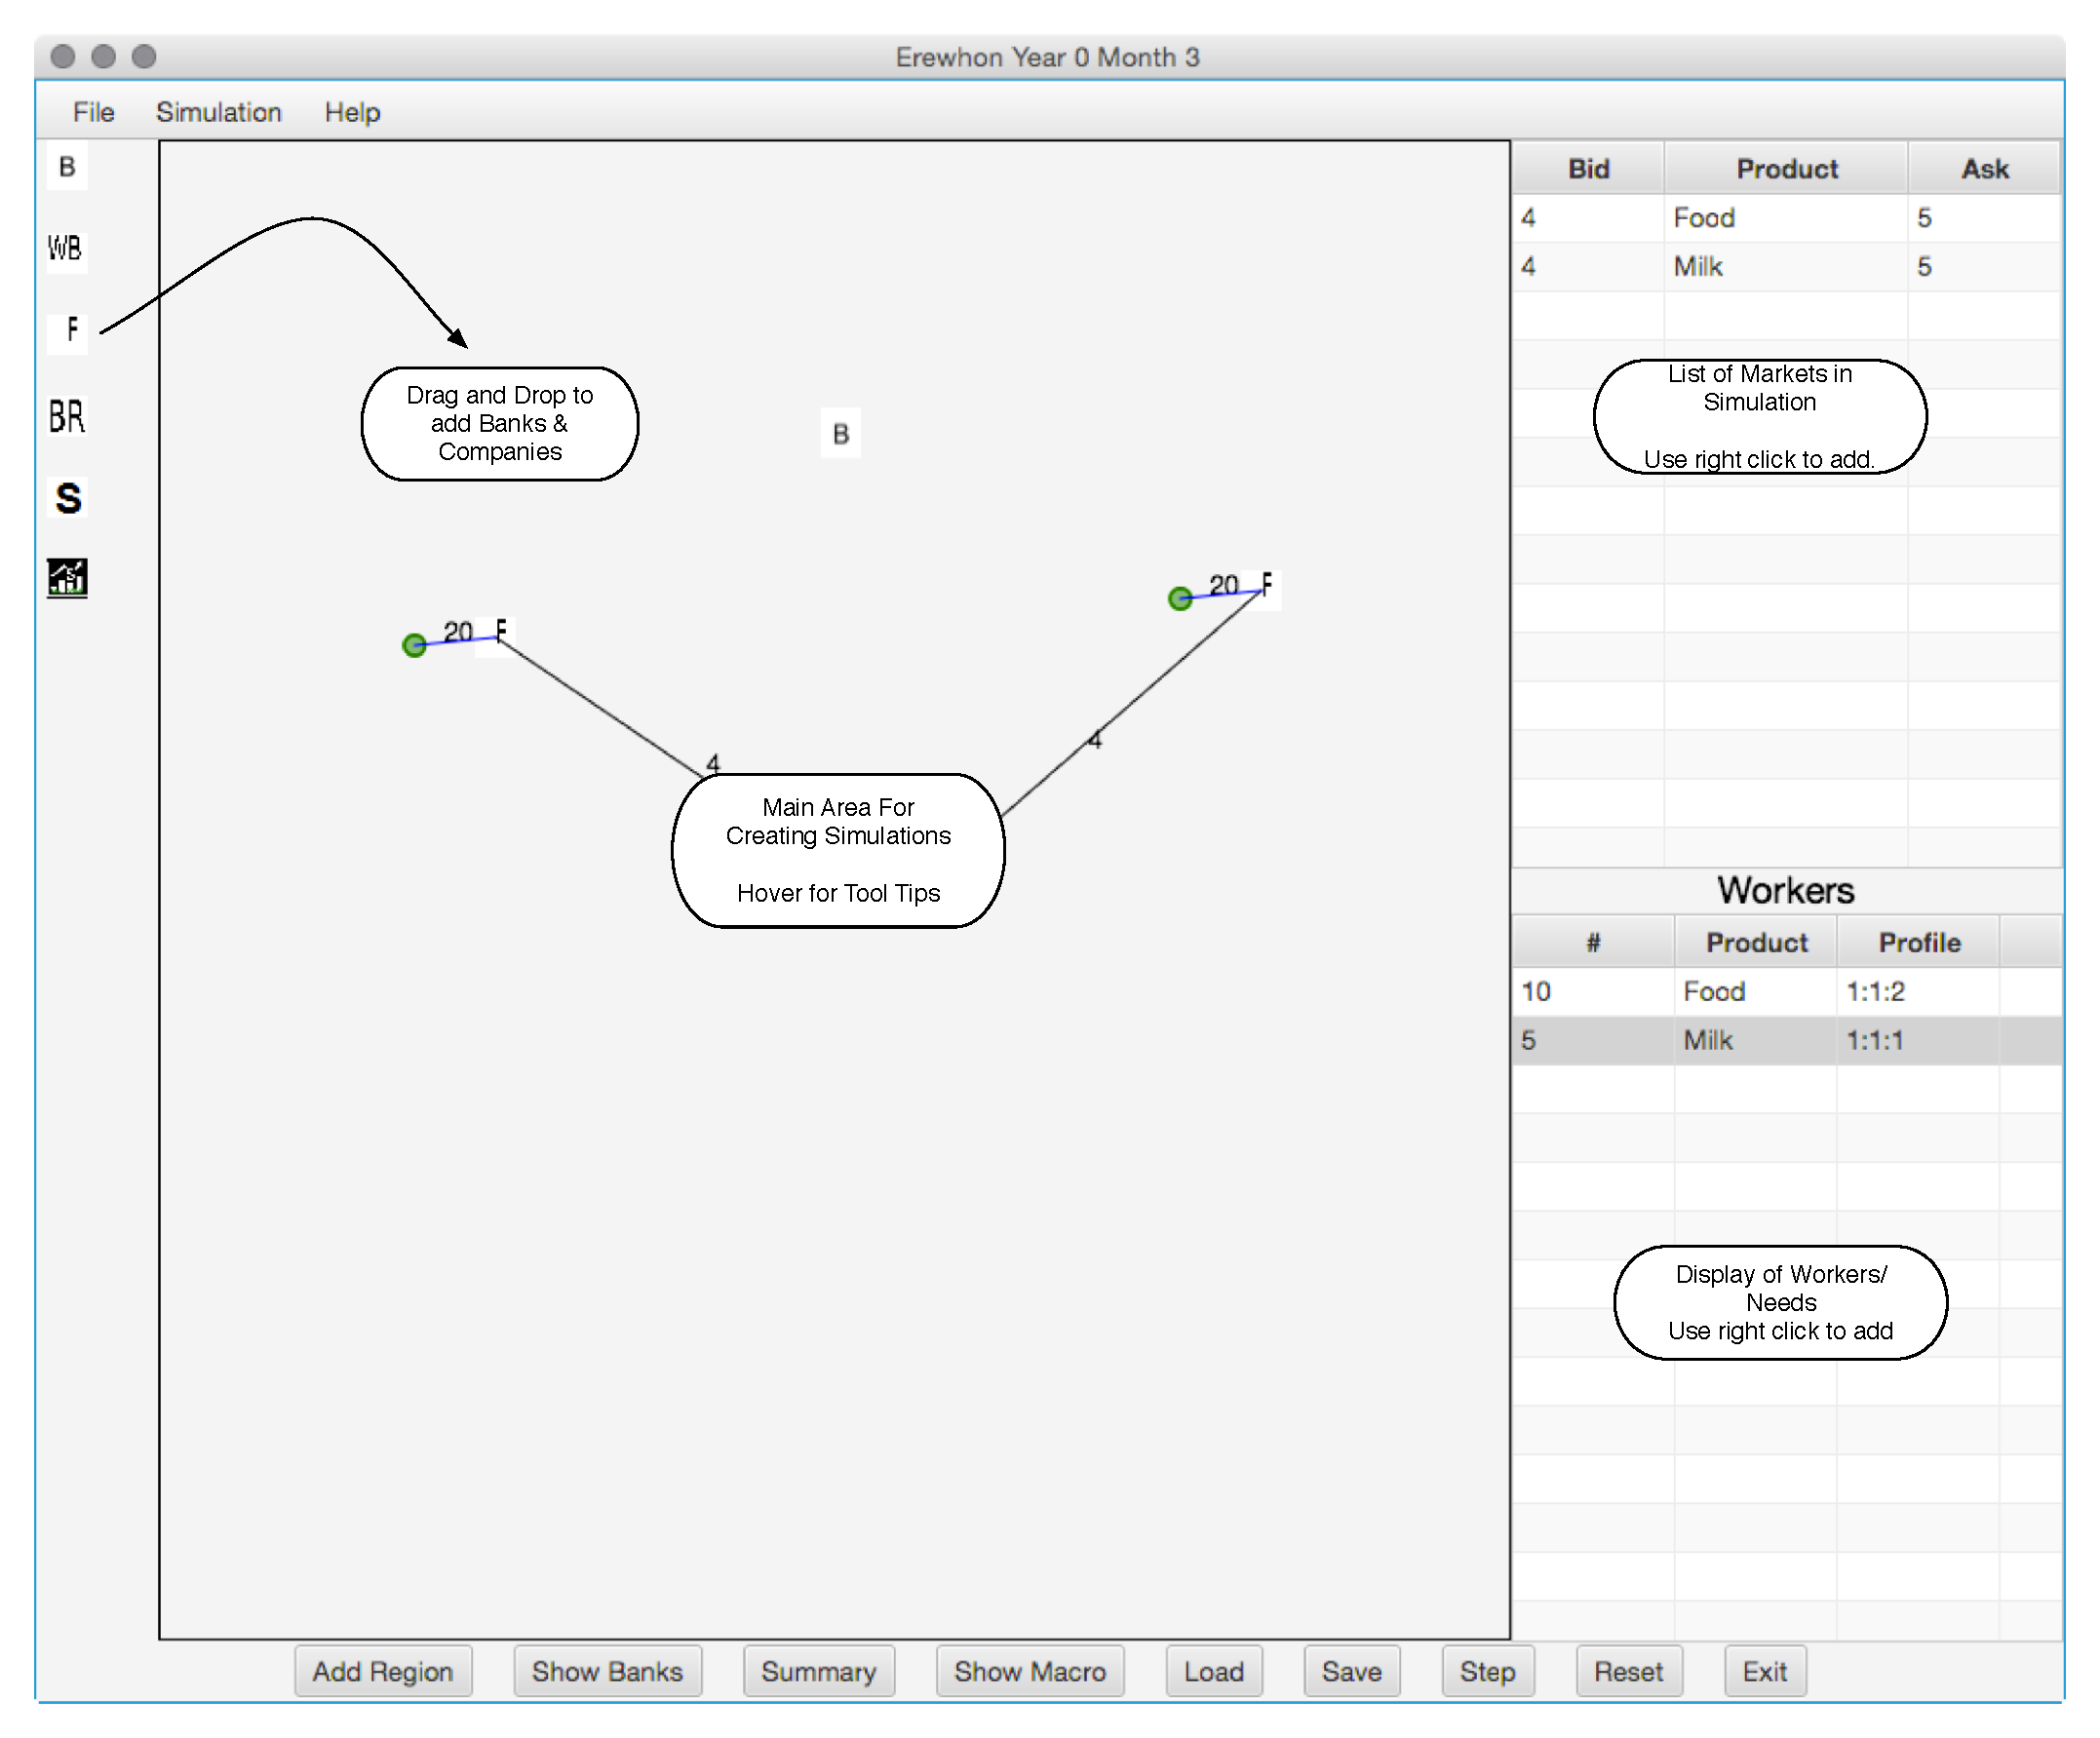
\includegraphics[width=14cm]{images/fig_mainScreen.eps}
\caption{Threadneedle Main Window}
\label{fig:mainscreen}
\end{center}
\end{figure}
A Threadneedle model is a description of an economic simulation to be
by the Threadneedle framework. It is an entity based set of
configuration descriptions which describes each individual accounting 
entity (agent) in the model. This description is then evaluated over time, 
according to the behaviours encapsulated by the java code of each
'agent' and the regulatory and tax framework set for the simulation. 
Economic parameters such as taxation, base interest rates, etc. can be
adjusted at any point during a simulation, and agents can also be
added if required.
\par
Each step in Threadneedle corresponds to a single day in a 30 days per
month, 360 day year - this is a simplification made primarily to ease
simulation analysis and debugging. (Extension to properly support the 
calender year may be considered in the future.)  
The title bar for the main screen displays the notional number of 
years, months and days
so far into the simulation. The Step button will run the simulation by one
or more steps at at time (rotate the button using scroll to select more steps), and
the Run and Stop buttons can be used to run the simulation continuously.
\par
Each simulation run is controlled by a configuration file or files. 
Configuration files are stored as editable json format 
files. In practice, small modifications can be made manually
to a configuration file, and slightly larger modifications can be made using tools
such as sed, but this is not the recommended way of
creating simulations. The graphical interface allows configurations
to be created, modified and inspected. Configurations can be saved and
loaded into the interface. Multiple configurations can be loaded into the simulation
from different files, provided they are consistent with each other. This 
provides a method of building partial configurations
that can be used as building blocks when creating multiple simulations.
\par
Default agents include banks, markets, producers, stock markets, workers
and investors. Agents can also be added to the simulation by extending
existing agents (See Programming Guide.). Several different financial
instruments are supported including compound, simple and Icelandic
indexed linked loans, Treasuries (government debt), securitized bank loans
and company shares. Loans can be arbitrarily specified with respect
to their duration, and the frequency with which payments are made.
\par
\subsection{Start}
The main start screen is shown in Figure \ref{fig:mainscreen}. Agents
can be added to the simulation by dragging and dropping from the
left hand bar, under agent specific menus on the right hand side, or directly
from the command line interface (see below). Tooltips
are available by hovering over items on the screen.
\par
All simulations must first define at least one  bank, as all agents 
in the simulation are required to have a bank account. Bank accounts will
be automatically created for agents when they are added to the simulation,
at the bank specified for the agent. When agents are being dragged and dropped
onto the main screen, the agent's account will be created at the bank physically closest to the agent.
\par
Once at least one bank is present, individual agents can be added to the simulation as required. There are some dependencies between agents, in 
particular producers need a market to sell their goods on, and producers
and workers need markets to buy goods from. These can be modified later, but 
the recommended order to create agents for the simulation to avoid this is:
\begin{enumerate}
\item Banks (At least 1 is required)
\item Markets 
\item Producers
\item Workers
\end{enumerate}
Markets are either added automatically on drag and drop if an agent
being added to the simulation requires one, or they can be added
manually by right clicking on the top right hand side menu and using
the Add Market dialog.
\begin{figure}[h]
\begin{center}
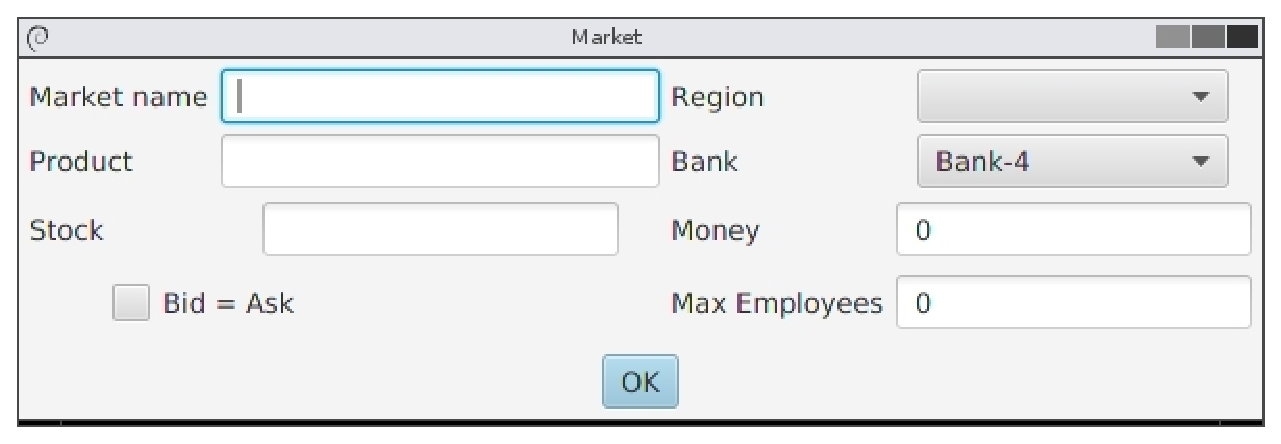
\includegraphics[width=14cm]{images/fig_addmarket.eps}
\caption{Add Market}
\label{fig:addmarket}
\end{center}
\end{figure}
Note, there are two places where workers can be added to the simulation,
the bottom right hand "Workers" section which creates workers who can
be hired from the labour market, and consume goods, and specialized
financial workers through the bank handling screens (See Banking below).
\par
Clicking on agents in the main display will bring up agent specific menus 
that allow their individual attributes to be modified.
\subsection{Banking}
A Central Bank will be automatically created with the Government, which
will also hold its account there.  Banks will use their reserve 
accounts at the central bank for clearing operations.\footnote{The exact mechanisms by which banks perform clearing is 
country and region specific, and has also varied considerably
over time. Today computerized 
Real Time Gross Settlement(RTGS) systems exist in most countries which 
typically use domestic banks accounts at their central bank for clearing. 
Separate systems can exist, major European inter-bank clearing operations 
are performed using the TARGET2 system, and clearing for small US banks can 
be done via local federal reserve banks. There are potential simulation
effecting liquidity considerations depending on exactly how this is
performed - for example historically it depended on physical exchanges,
requiring several days to process, and required higher reserves limits
than typical today, simply to handle the implicit buffering.}
\par
\subsubsection{Show Banks}
Once Banks have been added to the simulation, their ledgers can be
displayed using the "Show Banks" button at the bottom of the screen.
\begin{figure}[h]
\begin{center}
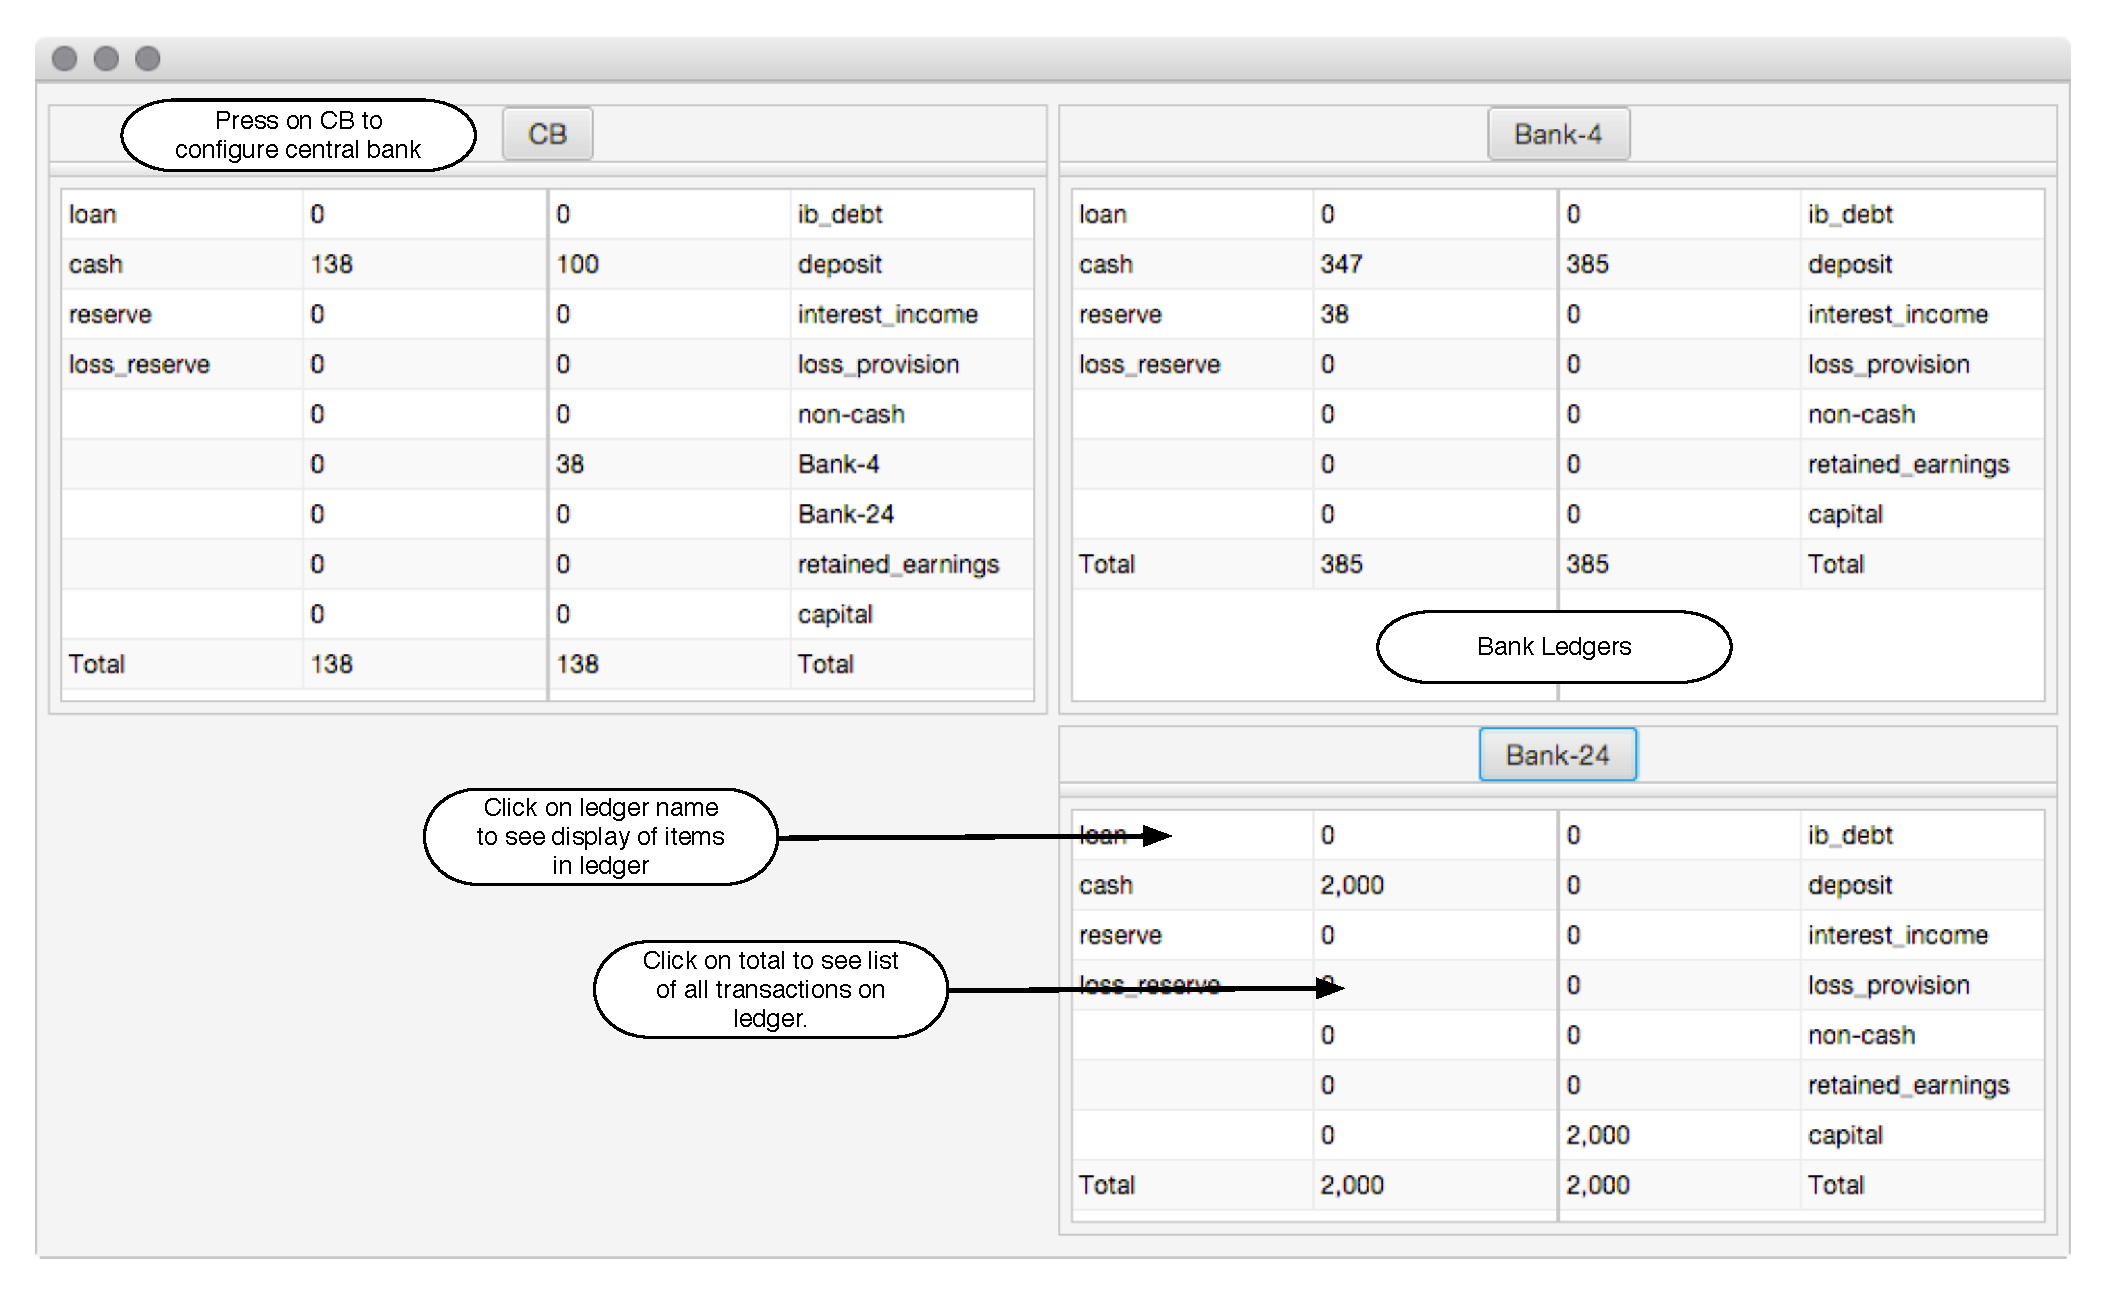
\includegraphics[width=14cm]{images/fig_banks.eps}
\caption{Show Banks}
\label{fig:banks}
\end{center}
\end{figure}
Ledgers are shown for each bank. Clicking on the bank's name will
bring up a dialog specific to that bank allowing 
interest rates, capital amounts etc. to be controlled, and account
holders to be added. 
\par
Clicking on the name of an individual bank's ledger will bring up a summary 
menu for the accounts or loans held by that ledger where this is appropriate.
Selecting the amount shown for the ledger will bring up the list of double
entry book keeping transactions that have been made to the ledger.
\par
All changes take effect in the step they are made. Changes can be
made during the simulation, for example to view the impact of 
interest rate changes on a given simulation banking system.
\subsubsection{Central Bank Configuration}
Selecting the central bank will show the dialog shown in Figure \ref{fig:centralbank}.
This dialog allows the 
reserve percentage and capital percentages for the banks controlled
by that central bank to be modified, and a base interest rate to 
be set for the simulation. Reserve and capital controls can be enabled and disabled
at will to see the impact on the simulation, or to explore simulations without
reserve controls, etc. The duration of an inter-bank loan (no. of steps) can
also be controlled. Changes to central bank parameters take immediate
effect within the model currently being simulated.
\begin{figure}[ht]
\begin{center}

\includegraphics[width=14cm]{images/fig_centralbank.eps}
\caption{Central Bank Configuration}
\label{fig:centralbank}
\end{center}
\end{figure}
\newpage
\subsubsection{Comercial Bank Configuration}
\par
\begin{figure}[ht]
\begin{center}
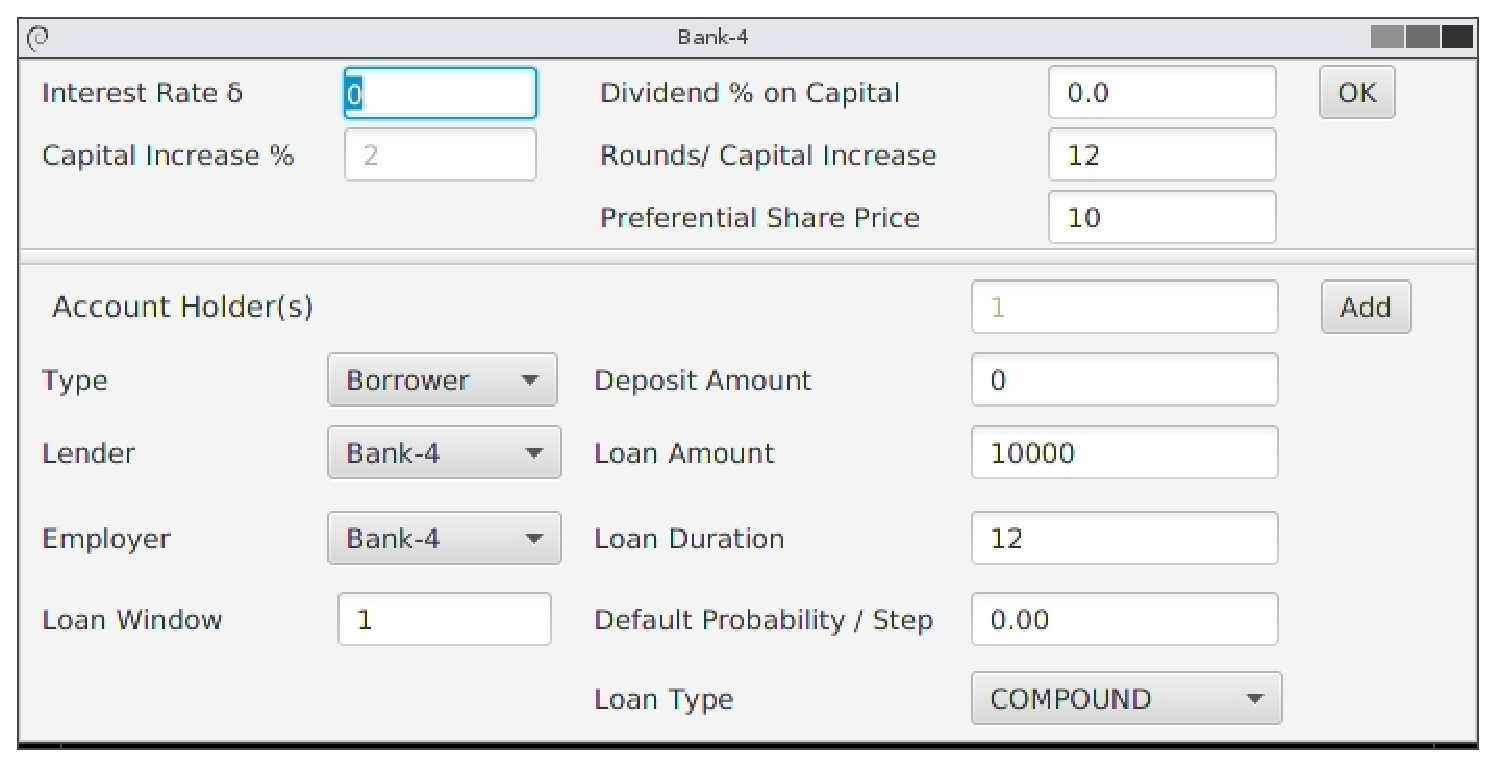
\includegraphics[width=14cm]{images/fig_bank.eps}
\caption{Individual Bank Configuration}
\label{fig:bank}
\end{center}
\end{figure}
\par
Figure \ref{fig:banks} shows the bank configuration dialog which can be
obtained by clicking on the individual bank's name. This allows 
different types of financial agent to be added to the simulation, 
and provides control over loan default rates, capital growth, and 
dividend payments for each bank individually. The following types
of account holder are currently supported:
\par
\paragraph{Borrower}
Borrowers are a special type of financial agent that provide a way to 
explore the banking system, decoupled from the rest of the economy. 
Borrowers attempt to take out loans for the amounts/periods/types specified
by the dialog, and then repay them. Borrowers are treated as bank employees,
in order to short circuit monetary flows from interest payments, and 
receive a salary from the bank that is sufficient to allow them to
meet their capital and interest payments, \emph{if, and only if} the bank
can afford to make these payments from its income.
\par
Which Bank employs the borrower can be set using the configuration 
dialog. Note that if borrowers are defined as receiving employment
from one bank, and a loan from a different one, then an asymmetric
flow of asset money will occur between the two banks. This can be
used to exercise the interbank lending mechanisms, and explore
related long term liquidity issues. 

\paragraph{Investor}
Investors provide an initial amount of asset cash, and receive
preferential shares which pay the dividend on capital specified
in the dialog for the bank. 
\begin{figure}[h]
\begin{center}
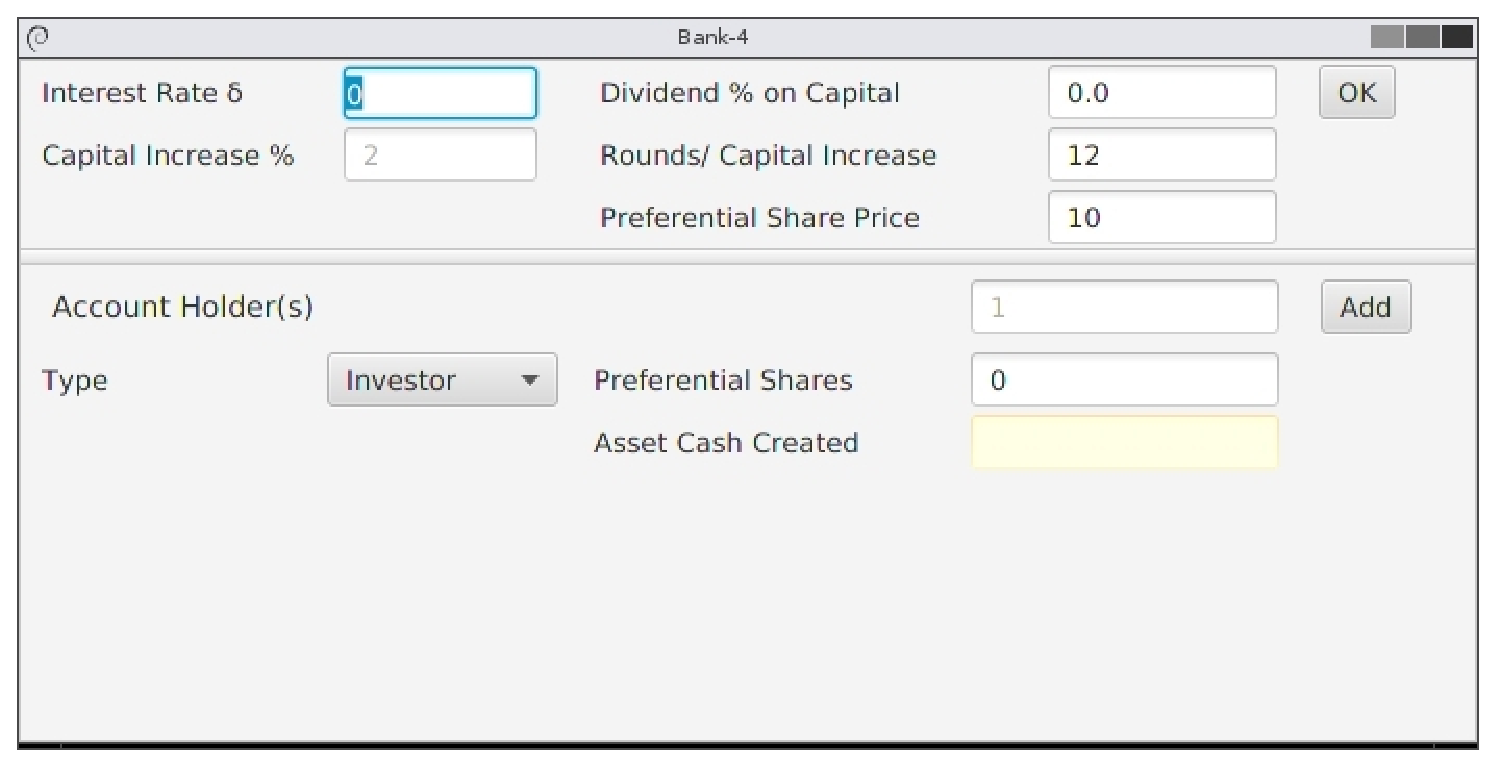
\includegraphics[width=14cm]{images/fig_investor.eps}
\caption{Account Holder:Investor}
\label{fig:investor}
\end{center}
\end{figure}
\paragraph{Saver}   
Savers provide asset cash, which is matched by a deposit at the bank
where they hold their account. They perform no other actions under
simulation - their main purpose is to provide initial liquidity, and
to facilitate experiments with 'stagnant' deposit money accounts in the banking
system. No interest is paid on these accounts.
\begin{figure}[h]
\begin{center}
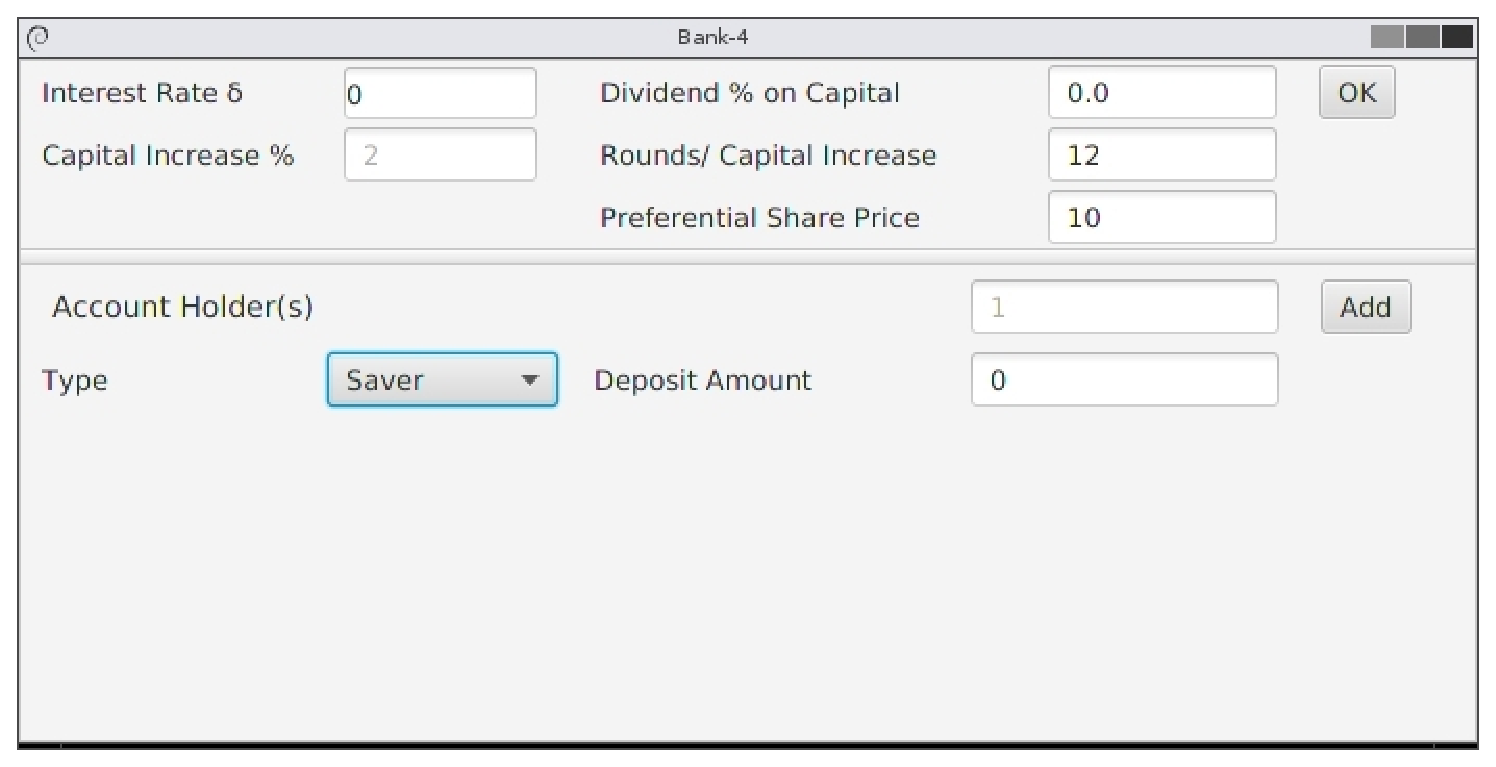
\includegraphics[width=14cm]{images/fig_saver.eps}
\caption{Account Holder:Saver}
\label{fig:saver}
\end{center}
\end{figure}

\subsubsection{Loan Types}
Individual Banks are currently restricted to issuing a single type of
loan, which is specified on configuration. The following loan types
are supported:
\begin{table}[ht]
\centering
\begin{tabular}{ll}
SIMPLE    & Fixed rate, simple interest loan   \\
COMPOUND  & Fixed rate, compound interest loan \\
ICELANDIC & Icelandic indexed linked loan      \\
\end{tabular}
\end{table}
\subsection{Charts}
A variety of charts are available to show the state of the simulation.
The charts being shown can be configured for each simulation by clicking
on the Charts display and selecting as appropriate. Additional
charts and statistics for display here can be added to the simulation 
if desired (See Programming Guide).
\begin{figure}[h]
\begin{center}
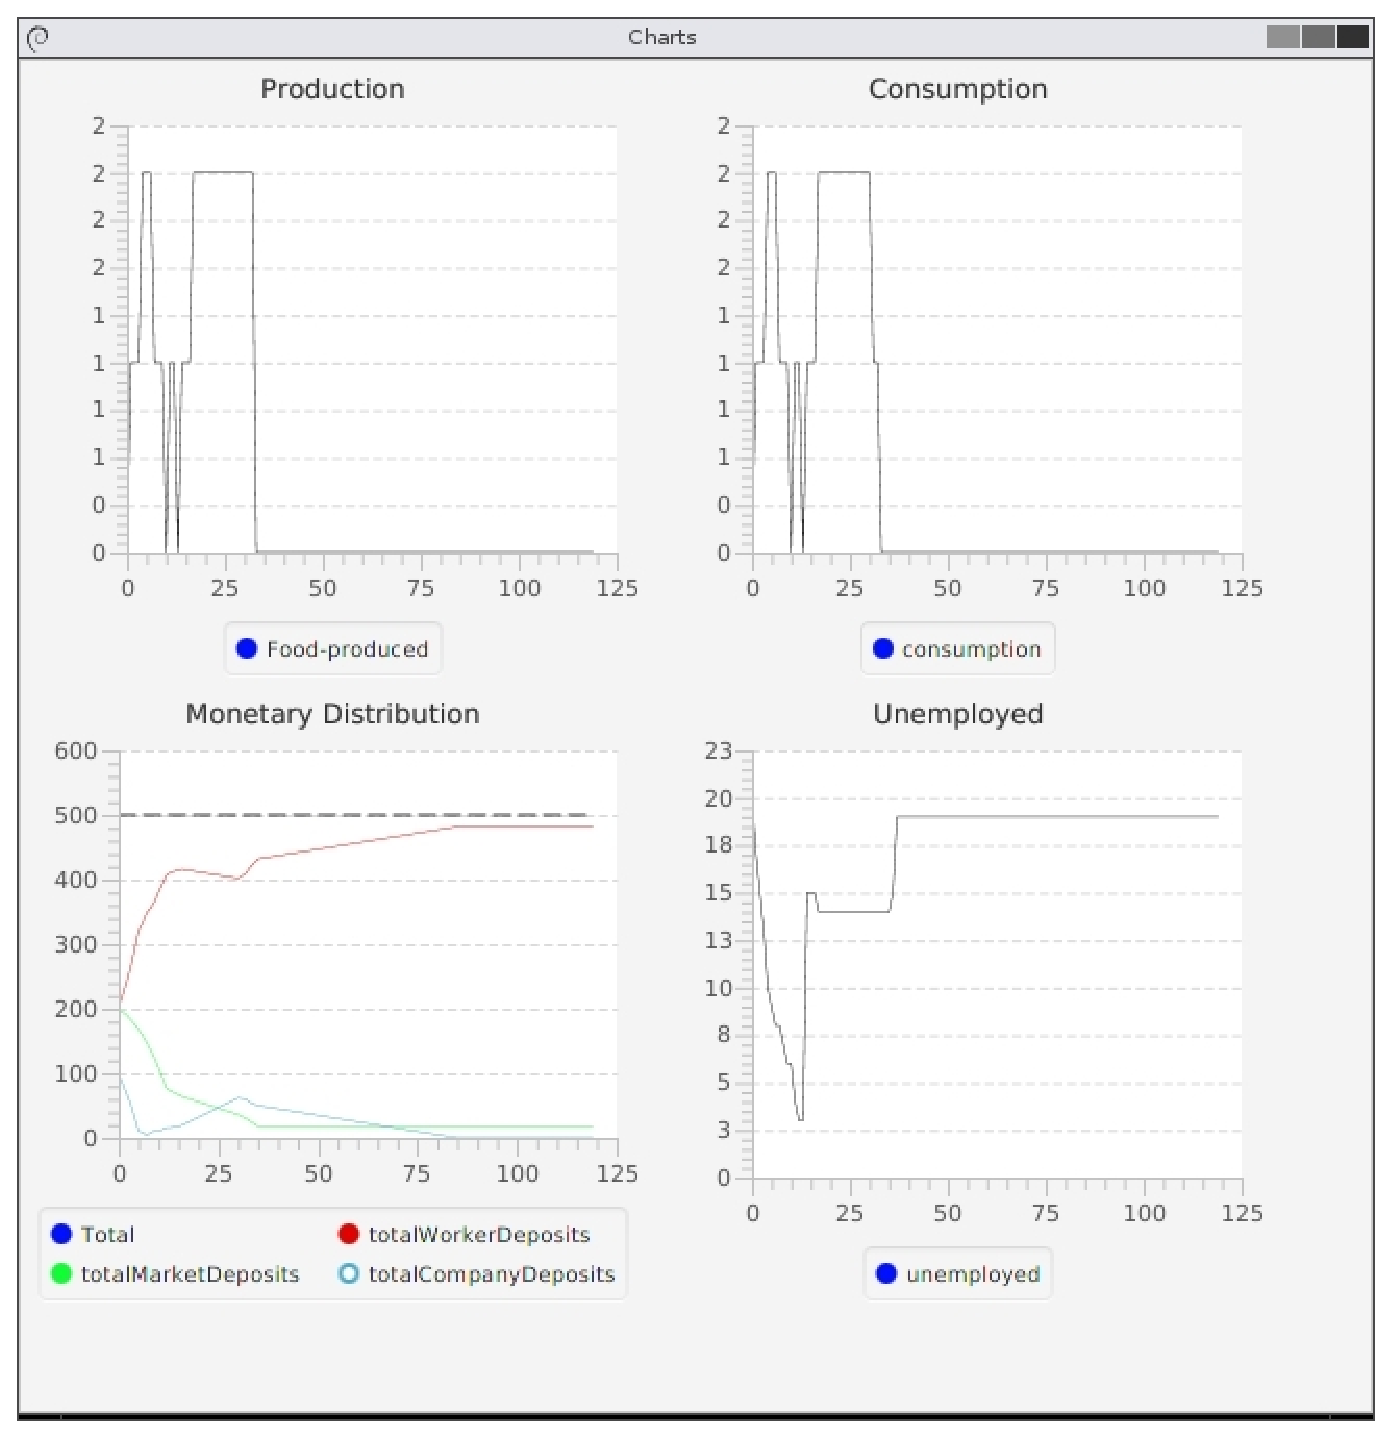
\includegraphics[width=14cm]{images/fig_charts.eps}
\caption{Simulation Charts}
\label{fig_charts}
\end{center}
\end{figure}

\chapter{Command Line Interface}
Threadneedle also provides a command line interface which can be
used to directly run and modify the active
simulation, as well as interact with batch mode.  To run with a command
line, use the option "-{}-cl" on startup, i.e.
\begin{description}[itemindent=3cm]
\item ./build \texttt{--cl}
\item ./run \texttt{--cl}
\end{description}

\subsubsection{help}
Print a summary of available commands.
\begin{center}
\begin{tabular}{c}
\begin{lstlisting}
> help
Commands: help
step [n]                 : Step simulation n steps (default 1200)
steps [n]                : Step simulation n steps while updating charts
repeat <times> <command> : repeat a command multiple times
forall <regex pattern> <command> : provide simple for loop capability
wait [time]              : wait a while before continuing reading commands
reset                    : reset simulation
set                      : set parameters in simulation
load <file>              : load new config file
preferences <filename>   : load Threadneedle parameters from file
config                   : show current parameters for simulation
statistics               : show statistics registered with simulation

printmoney agent x     : increase agent's deposit by x
addagent <type> <bankname> [options] : add an agent with [options] as properties key=value map
agentinfo <agent>      : invoke toString() on <agent>
debug [file]           : toggle debugging information on and off
agentinfo <agent>      : invoke toString() on <agent>
htmlcharts [dir]       : write charts out in html/png format
report [file]          : print report on simulation optionally to file
setbaserate            : change the base interest rate
shareholders <stockmarket> : print the shareholders of the given stockmarket
savechartdata [dir]        : write chart's series data out to a file for that chart as png

savechartcsvdata [dir] : write chart's series data out to a file for that chart as csv
printorders <agent>    : print the orders listed on stockmarket <agent> or put up by <agent>
quit               : exit simulation

\end{lstlisting}
\end{tabular}
\end{center}
%
\subsubsection{report [file]}
Print a report of the simulation results, optionally to a named
file.
%
\subsubsection{htmlcharts directory}
Write charts specified for the simulation to the specified directory
in png format. Directory will be created if it does not already 
exist, and existing charts files will be overwritten.
\subsubsection{htmlsetup directory}
Write a simplified report of the simulations configuration 
to a file called $test_config$ in the specified directory. This
will be automatically displayed by the Threadneedle.php page
if this has been setup.
\subsubsection{addagent}
Add an agent to the model. An initial deposit must be specified,
other parameters for the agent can be passed in as strings. For example:
\begin{center}
\begin{tabular}{c}
\begin{lstlisting}
addagent <type> <bankname> initialDeposit=X [options]
eg.
addagent Person Bank-4 initialDeposit=50
addagent Farm   Bank-4 initialDeposit=100 labourInput=3
\end{lstlisting}
\end{tabular}
\end{center}
\subsubsection{addneed/addwant}
\begin{center}
\begin{tabular}{c}
\begin{lstlisting}
addneed agent-id name purchase consume store consumable useLoan
eg.
addneed Person-60 Food 1 1 1 true false
\end{lstlisting}
\end{tabular}
\end{center}
Associates a need or a want with a specified agent.
\subsubsection{set}
Set parameters in the active simulation's configuration. Note, these
will not affect the simulation's behaviour until the simulation
is reset using the reset command and run from the beginning. The
format of the set command is:
\begin{center}
\begin{tabular}{c}
\begin{lstlisting}
set <agent name> <parameter> <value>
eg.
set A0 initialDeposit 20
\end{lstlisting}
\end{tabular}
\end{center}
%
\subsubsection{forall}
The forall command provides a limited looping capability that
can be used in conjunction with other commands. The format
of the command is:
\begin{center}
\begin{tabular}{c}
\begin{lstlisting}
forall <regex pattern> <command>       
e.g.
forall ^A set initialDeposit 15
\end{lstlisting}
\end{tabular}
\end{center}
will set all the initial deposit for all agents whose name begin
with A to 15. 
\subsubsection{printmoney}
The printmoney command can be used while the simulation is running
to increase the money supply by increasing an agent's deposit
at the bank. At present this only works in constant money 
supply simulations (those using the simple Bank class), since
double entry book keeping prevents agent's deposits being
arbitrarily increased within a fractional reserve framework
without side effects.  The format command is:
\begin{center}
\begin{tabular}{c}
\begin{lstlisting}
printmoney <agent name> <amount>
e.g.
printmoney A0 300
\end{lstlisting}
\end{tabular}
\end{center}
\subsubsection{reset}
Reset the simulation state to that of the configured parameters.
This will cause any changes made by the set command to take
effect.
\subsubsection{step}
Step the simulation a specified number of steps.
\subsubsection{quit}
Exit the simulation.
\section{Command line interface and Batch Mode}   
Threadneedle provides a batch mode which allows
experiments to be run from either the command line, batch command files or
a combination of both. Graphs 
and results showing the results of these experiments can be saved to a 
user controlled directory for later viewing, as well as being displayed
during the batch run.
\subsection{Connection between batch and config files}
A batch file provides a series of commands that are executed
sequentially on the simulation described by the configuration 
file Threadneedle is invoked with. There is no connection between
the batch file and the configuration file beyond the requirement that
the commands in the batch file can be applied to the agents specified in the 
configuration file. 
\par
The commands available from a batch file are the same as those available from the
Threadneedle command line, and can be seen by using the "help" command
on the Threadneedle command line.
\subsection{Comments}
In both the configuration file and the batch file, a \# symbol at the
beginning of the line can be used to add comments to the file
\subsection{Running in batch mode}
The command is:
\par
\bigskip
\mbox{java -classpath "classes:src/resources:lib/*:" gui.Threadneedle --b=<filename>}

Optionally the "--charts" option can be supplied to view the simulation's 
chart information without displaying the main simulation screen. An RNG seed can
also be specified.

\section{Web Integration}
To facilitate viewing the results from multiple experiments a \emph{node.js}
server is provided which allows a web browser to easily view the
results of experiments. 

The chartserver.js file can be found in the ../Threadneedle directory. By
default the server uses the contents of the \emph{output} directory in
the directory it is run from, and
the results can viewed using a webbrowser from the url \url{127.0.0.1:1234}.
To run the node.js server use the command:
\par
\bigskip
\begin{center}
\mbox{node chartserver.js}
\end{center}

Reloading the webpage
pointing at \url{127.0.0.1:1234} will then cause the server to automatically
cycle between the charts in the market1 and market2 output directories.

Chart images can be created in batch (or from the command line) by using the
htmlsetup and htmlcharts commands. For example, the following batch
file will load the market1.json configuration file, run it for 100
steps, save the charts to output/market1 and then run for another 100
steps before saving the charts to output/market2. 

\begin{center}
\begin{tabular}{c}
\begin{lstlisting}
load configs/market1.json
debug off
step 100
htmlsetup output/market1/
htmlcharts output/market1/
step 100
htmlsetup output/market2/
htmlcharts output/market2/
\end{lstlisting}
\end{tabular}
\end{center}
%\chapter{Sample Experiments}
%
% - Show expansion constrained by number of borrowers
%   Max lending is N borrows * Loan Amount (over all banks)
%
\chapter{Known Problems}

\end{document}
